\documentclass[a4paper,11pt]{article}
\usepackage[spanish]{babel}
\usepackage[utf8]{inputenc}
\usepackage[margin=3.5cm]{geometry}
\usepackage{setspace}
\usepackage{tipa}
\usepackage{amssymb}
\usepackage{listings}
\usepackage{graphicx}
\usepackage{float}
\usepackage{hyperref}
\usepackage{fancyhdr}
\usepackage{multirow}
\usepackage{amsmath} 
\usepackage{amsthm}
\usepackage{color,graphicx}
\usepackage{algorithm}
\usepackage{algpseudocode}
\usepackage{amsmath}
\usepackage{pdfpages}
\usepackage{caption}
\usepackage{subcaption}
\usepackage{tcolorbox}
\usepackage{color}
%\usepackage{dsfont}

\definecolor{mypink}{HTML}{F9F2F4}

\setlength{\headheight}{14pt}
\linespread{1.2}
\definecolor{javared}{rgb}{0.6,0,0} % for strings
\definecolor{javagreen}{rgb}{0.25,0.5,0.35} % comments
\definecolor{javapurple}{rgb}{0.5,0,0.35} % keywords
\definecolor{javadocblue}{rgb}{0.25,0.35,0.75} % javadoc
\lstset{language=Java,
basicstyle=\ttfamily,
keywordstyle=\color{javapurple}\bfseries,
stringstyle=\color{javared},
commentstyle=\color{javagreen},
morecomment=[s][\color{javadocblue}]{/**}{*/},
numbers=left,
numberstyle=\tiny\color{black},
stepnumber=0,
numbersep=10pt,
tabsize=4,
showspaces=false,
showstringspaces=false}

\newcommand{\nemph}[1] { \textbf{\emph{#1}}}
\newcommand{\redbox}[1] { \colorbox{mypink}{\textcolor{red}{#1}}}

\begin{document}
    \title{COMPUTACIÓN CONCURRENTE \\ { PRÁCTICA 2, PRIMITIVAS DE SINCRONIZACION}}
    \author{
    	Prof. Manuel Alcántara Juárez \\
    	\texttt{manuelalcantara52@ciencias.unam.mx}
    	\and
    	Leonardo Hernández Cano \\
    	\texttt{leonardohernandezcano@ciencias.unam.mx}
    	\and
    	Ricchy Alain Pérez Chevanier \\
    	\texttt{alain.chevanier@ciencias.unam.mx}}
    \date{Fecha Límite de Entrega: 13 de Septiembre de 2019 a las 23:59:59pm.}
    
	\maketitle
	\pagestyle{fancy}

	\fancyhf{}
	\fancyhead[l]{Práctica 02} 
	\fancyhead[r]{Computación Concurrente}
	\fancyfoot[c]{\thepage}
	
	\section{Objetivo}
	El objetivo de esta práctica es implementar algunos algoritmos de sincronización vistos en clase y una aplicación del uso de las primitivas de sincronización que construiste mediante estos algoritmos.
	
	\section{Desarrollo}
	En esta práctica trabajarás con una base de código construida con Java 8\footnote{De nuevo puedes utilizar cualquier versión de java que sea mayor o igual a Java 8 simplemente ajustando el archivo pom.xml}  y Maven 3, también proveemos pruebas unitarias escritas con la biblioteca \verb|Junit 5.5.1| que te darán retrospectiva inmediata sobre el correcto funcionamiento de tu implementación\footnote{Bajo los casos que vamos a evaluar, mas estas no aseguran que tu es implementación es correcta con rigor formal} . \\
	Para ejecutar las pruebas unitarias necesitas ejecutar el siguiente comando: \\
	
	\begin{tcolorbox}
		\begin{lstlisting}
$ mvn test
		\end{lstlisting}
	\end{tcolorbox}

	Para ejecutar las pruebas unitarias contenidas en una única clase de pruebas, utiliza un comando como el siguiente: \\
	
	\begin{tcolorbox}
		\begin{lstlisting}
$ mvn -Dtest=PetersonLockTest test
		\end{lstlisting}
	\end{tcolorbox}

	En el código que recibirás la clase \verb|App| tiene un método \emph{main} que puedes ejecutar como cualquier programa escrito en \emph{Java}. Para eso primero tienes que empaquetar la aplicación y finalmente ejecutar el jar generado. Utiliza un comando como el que sigue: \\
	
	\begin{tcolorbox}
		\begin{lstlisting}
$ mvn package
... 
...
$ java -jar target/practica02.jar
		\end{lstlisting}
	\end{tcolorbox}

	\section{Evaluación}
	Además de que tu código pase las pruebas unitarias sin que estas hayan sido modificadas, también debes de escribir una justificación breve de por qué tu solución cumple con las propiedades requeridas en la descripción del problema, añade estas justificaciones al inicio de cada clase o como pequeños comentarios intermedio dentro de tu implementación.
	
	\section{Problemas}

	\subsection{Algoritmo de Peterson}
	Para esta actividad tienes que implementar el algoritmo de Peterson visto en clase para generar un \emph{candado} que solucione el problema de la exclusión mutua para dos hilos. En el código fuente que acompaña a este documento encontrarás la clase \verb|PetersonLock| que implementa la interfaz \verb|Lock|, tu tarea es completar la implementación de esta clase. Para validar que tu implementación es correcta tienes que pasar todas las pruebas unitarias que se encuentran en la clase \verb|PetersonLockTest|.
	
	\subsection{Algoritmo del Filtro}
	Utilizando la idea del \verb|Algoritmo del Filtro| visto en clase, crea una implementación que permita pasar a lo más a \( L \) hilos a su sección crítica con \(L < N\).  Completa la implementación de la clase \verb|FilterSemaphoreImpl|, para verificar que tu implementación funciona tienes que pasar todas las pruebas unitarias que se encuentran en la clase \verb|FilterSemaphoreTest|.

    \subsection{El Problema de los Filósofos}
    El problema de los filósofos fue inventado por E. W. Dijkstra, un pionero de la concurrencia, para clarificar la noción de algoritmos libres de \nemph{abrazos mortales} y de \nemph{hambruna}. Imagina cinco filósofos que sólo pasan su vida pensando y comiendo. Ellos se sientan alrededor de una mesa redonda con cinco sillas. La mesa tiene cinco platos grandes de arroz, sin embargo, solamente hay cinco palillos disponibles (un poco insalubre), como se muestra en la figura. Cada filósofo piensa, luego le da hambre, por lo que se sienta y toma los dos palillos que se encuentran a su lado. Si el filósofo pueda tomar ambos palillos, entonces procede a comer por un rato. Una vez que el filósofo termina de comer, éste regresa los palillos al lugar de donde los tomó y de nuevo se pone a pensar.\\
    
    \begin{figure}[!ht]
		\centering
		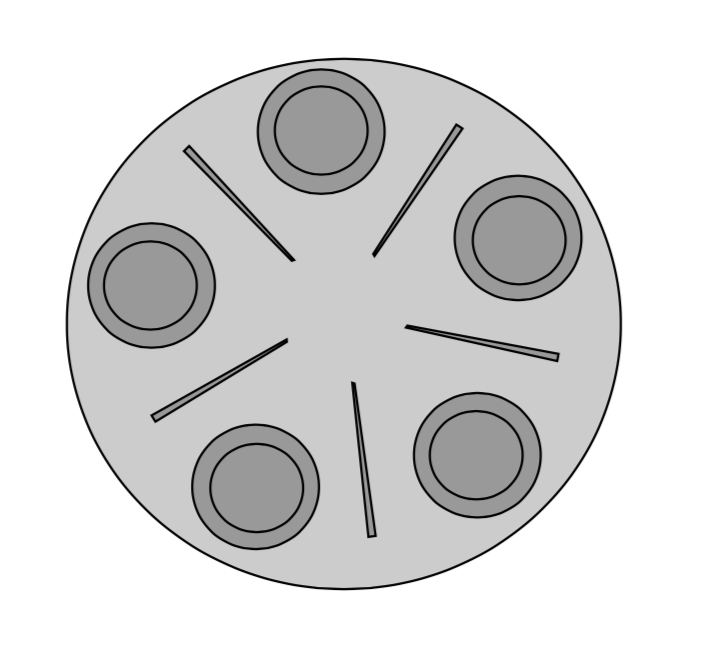
\includegraphics[width=0.5\textwidth]{./imgs/dining-table.png}
	\end{figure}
    
    Para la solución a las siguientes actividades solo puedes utilizar primitivas de sincronización que tú mismo implementes, no puedes utilizar las que proporciona el \emph{API} de \verb|Java|. Realiza las siguientes actividades:
    
    \begin{enumerate}
		\item{Termina de implementar la clase \verb|ChopstickImpl|, la idea es que puedas asegurar que este objeto no puede ser tomado por más de un hilo simultáneamente. Para verificar que tu solución es correcta necesitas pasar todas las pruebas unitarias que se encuentran en la clase \verb|ChopstickTest|.
		}
		\item{Tu siguiente tarea es completar la implementación del problema de los filósofos, dicha implementacion tiene que cumplir las siguientes 3 características:
		    \begin{enumerate}
		        \item{Los cinco filósofos interactúan concurrentemente en la mesa, compitiendo por tomar los palillos para comer.}
		        \item{La simulación es libre de \emph{abrazos mortales}.}
		        \item{La implementación es libre de \emph{hambruna}.}
		    \end{enumerate}
		    En el código fuente encontrarás dos clases \verb|Philosopher| y  \verb|PhilosopherWIthFilterAlgorithm|, estas son las que tendrás que completar para poder pasar las pruebas unitarias que se encuentran en la clase \verb|PhilosopherTest|.\\
		    Para solucionar este problema puedes utilizar las siguientes estrategias:
		    \begin{enumerate}
				\item{Modifica la clase \verb|PhilosopherWIthFIlterAlgorithm| para que a lo mas 4 filósofos puedan comer al mismo tiempo en ella por medio de un semáforo, utiliza la implementación de semáforos que creaste en el ejercicio 3.1.}
		    \end{enumerate}
		    }
		
	\end{enumerate}

\end{document}
